%
% Transportation Research Board conference paper template
% version 3.1 Lite
%
% When numbered option is activated, lines are numbered.
\documentclass[numbered]{trbunofficial}
\usepackage{graphicx}
%\usepackage{cite}
\usepackage{amsmath,amssymb,amsfonts}
\usepackage{algorithmic}
\usepackage{graphicx}
\usepackage{textcomp}
\usepackage{xcolor}
\usepackage{multirow}
\usepackage{pdflscape}
\usepackage{afterpage}
\def\BibTeX{{\rm B\kern-.05em{\sc i\kern-.025em b}\kern-.08em
    T\kern-.1667em\lower.7ex\hbox{E}\kern-.125emX}}

% \usepackage[colorlinks=true,linkcolor=blue,citecolor=blue]{hyperref}
% For TRB version hide links
\usepackage[hidelinks]{hyperref}

\makeatletter
\renewcommand\@biblabel[1]{#1.}
\makeatother

% Put here what will go to headers as author
\AuthorHeaders{Brown, Garikapati and Hou}
\title{A Machine Learning Decision Support Tool for\ \ \ \ \ \ \ \ \ \ \ \ \ \ \ \ \ \ \ \ \ \ \ \ \ \ \ \ \ \ \ \ \ \  Travel Demand Modeling}

% TODO: add macros for easier formatting of \author.
\author{%
  \textbf{TRB Paper - 19-04806}\\
  \hfill\break%
  \hfill\break%
  \textbf{CScott Brown}\\
University of South Alabama\\
Email: gitpushoriginmaster@gmail.com\\
  \hfill\break%
  \textbf{Venu M. Garikapati, Ph.D}\\
National Renewable Energy Laboratory\\
15013 Denver West Parkway, Golden, Colorado 80401\\
Tel: 303-275-4784\\
Email: venu.garikapati@nrel.gov\\
  \hfill\break% this is a way to add line numbering on empty line
  \textbf{Yi Hou}\\
National Renewable Energy Laboratory\\
15013 Denver West Parkway, Golden, Colorado 80401\\
Tel: 303-384-7525\\
Email: yi.hou@nrel.gov \\
}

% If necessary modify the number of words per table or figure default is set to
% 250 words per table and figure
% \WordsPerTable{250}
% \WordsPerFigure{250}

% If words are counted manually, put that number here. This does not include
% figures and tables. This can also be used to avoid problems with texcount
% program i.e. if one does not have it installed.
\TotalWords{1739}

\begin{document}

\maketitle

\section{Introduction} \label{section:introduction}

Utility maximization models are the lifeblood of virtually all travel demand models in practice. 
 Be it the traditional travel demand models or more advanced activity-based models, utility maximization models are used extensively to model and predict myriad travel choices such as location choice, mode choice and route choice. 
 However, there is increasing interest in incorporating machine learning (ML) into travel demand models to enhance prediction accuracy, and because ML techniques often require less stringent assumptions on, for example, variable error distributions than traditional statistical modeling methods.
 In the transportation field, ML is gaining rapid popularity in driver behavior modeling \trbcite{meng2012classification}, travel time prediction \trbcite{hou2017road}, traffic forecasting \trbcite{ma2015large}, volume estimation \trbcite{hou2018network}, and safety analysis \trbcite{brijs2007bayesian, miranda2007bayesian}. 
 There has been a great deal of effort in comparing utility maximization models to specific classes of ML models in specific contexts.
 However, these efforts give mixed and sometimes contradictory results, and are largely incomparable due to the complexity of ML models and the inherent latitude available to an investigator in model design and evaluation attendant to it.
 Thus, there is a need for a standardization in evaluation of ML models against utility maximization models for a given choice context. 
 
Notably, in the context of mode choice modeling: 
 Zhang et al \trbcite{zhang2008travel} perform a comparison of Support Vector Machine (SVM), Multilayer Perceptron (MLP) (a subset of neural networks) and Multinomial Logit (MNL) models and find that SVM models have a slight edge. 
 Xie et al \trbcite{xie2003work} compare Decision Tree (DT), MLP and MNL models finding that the Decision Tree and MLP models perform somewhat better.
 However, Vythoulkas et al \trbcite{vythoulkas2003modeling} also compare MNL with a Neural Network architecture but find that there is no meaningful difference in their performance.
 Further, Hagenauer et al \trbcite{hagenauer2017comparative} compare a number of model families and find a significantly greater difference between performance of ML models and MNL models than previous studies.
 Unfortunately, these studies are quite different in model design, even for the same model families, and because they take different approaches to evaluation, they are impossible to objectively compare.
 Similar observations can be made in the literature on ML model design and evaluation for other variables frequently used in travel demand models.

Addressing the need for standardization and to provide a means by which models may be more easily compared, we present a tool for applying an array of models including MNL, Nested Logit (NL), MLP, Naive Bayes (NB), Ordinal Probit (OP) and Random Forest (RF) classifiers. 
 The tool (TEAM-TDM \ref{fig:flowchart}) is designed to be easily extensible, accounts for common pitfalls in the application of various models, automatically selects optimum hyperparameters and reports a variety of metrics commonly employed to evaluate model performance. 
 The tool is specifically tailored to aid in deciding the best model for a given choice context and can be used to choose an appropriate model family or to construct a model ensemble. 
 Results demonstrate that for some variables, MNL are not the most effective models, and the proposed system can aid in selecting a better model.
 The goal of our experiments is to provide a unified framework that can be applied to a variety of problem sets, allowing practitioners and researchers to easily and fairly compare the performance of different model families on individual tasks, but also between tasks.

\begin{figure}[!ht]
  \centering
  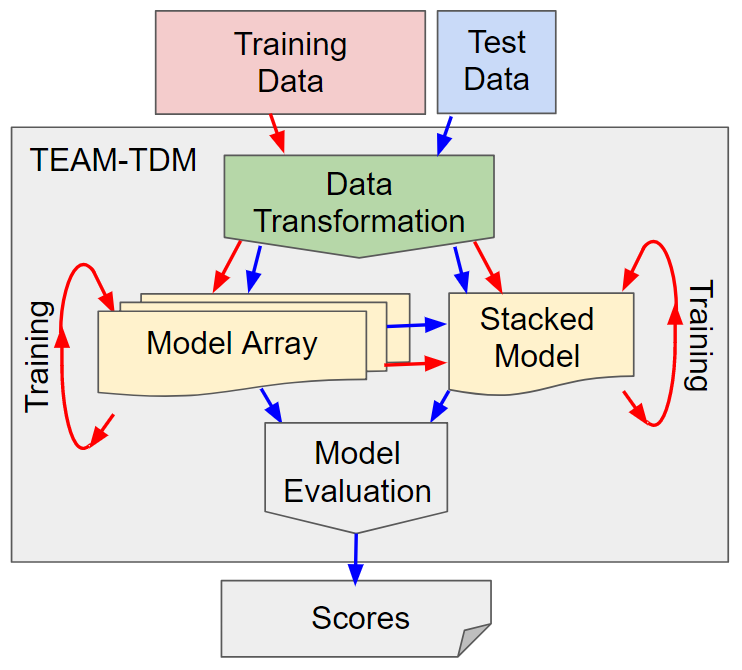
\includegraphics[width=0.6\textwidth]{flowchart}
  \caption{The TEAM-TDM tool.}\label{fig:flowchart}
\end{figure}



\section{Methodology} \label{section:introduction}

We test our proposed system on household vehicle count and work schedule targets from the 2017 National Household Travel Survey.
 In applying the tool to these datasets, we apply TEAM-TDM in an identical configuration.
 Thus, the experiments show that TEAM-TDM can be meaningfully applied to myriad classification problems in the transportation domain.

The tool itself can include arbitrary model families, but for comparison purposes we include in the evaluation on both problems MNL, RF, MLP and NB classifiers.
 In addition to training the models, TEAM-TDM preprocesses the data by performing scaling, feature selection and dummy variable introduction.
 It also chooses optimum hyperparameters for the given model families using bayesian optimization on cross-validation accuracy.
 Finally, TEAM-TDM provides a variety of performance metrics, allowing evaluation of models according to a number of real-world criteria.
 Lastly, the tool trains a `stacked' model which combines the individual models in an attempt to maximize the overall accuracy.

Since the tool performs the entire data processing, model training and evaluation pipeline, one can apply it to different problem sets with nearly zero effort.
 As such, we apply the tool to the prediction of household vehicle count and work schedule targets from the 2017 National Household Travel Survey using the absolute minimum possible user intervention (such as identification of categorical variables).
 In this way, the experiments are designed to show that a unified pipeline can be applied to different problems, resulting in evaluations that can be easily compared across model families and datasets.
 In addition, the experiments are designed to show that this same unified pipeline produces models that perform comparably to prior research, so that TEAM-TDM gives reasonable models.

\section{Findings} \label{section:results}

\subsection{NHTS household vehicle ownership prediction}\label{subsection:vehicle}

The target feature for this exercise is the number of vehicles owned by the household.
 All of the models in our experiments are capable of accounting for weighted data, which we include in our training pipeline.
 Besides the row identifiers, the weights, and the target, we initially include all features in our training pipeline, and let the model decide which are important.
 Table \ref{table:features} includes some summarizing statistics of various variables in the NHTS 2017 household-level dataset.

Model scores are summarized in the first section of Table \ref{table:results}.
 Since vehicle count admits an ordinal interpretation, and since additional model families can be included into TEAM-TDM as a parameter, we include an OP and an NL model for comparison.
 This allows for an indirect comparison with prior results along the same vein.
 For example, in \trbcite{bhat1998comparison}, MNL and Ordinal Logit (devised using a different nesting structure than ours) give best case accuracies of around $59\%$.
 This is comparable to the results of our MNL and OP models and suggests that TEAM-TDM produces model results that are comparable to similar studies in the field.
 Note that the inclusion of these additional model families does not affect the results of other model families, and thus does not preclude a comparison of models between our two datasets.

The NL model seems to perform best, although the MLP and OP models are not far behind.
 Since the MLP does not benefit from our a priori knowledge of ordinality in the target variable this might reasonably be expected.
 The RF model performs comparably to the MLP model.
 Another interesting observation is that the NL model trains significantly faster than the MNL model, even though both utilize the same libraries for logit modeling.
 This fact, along with the good performance of the MLP model, suggest that a nested MLP or RF model might be worth exploring further in the context of vehicle ownership models.

The stacked model performs even better than the NL model across the board but requires a significant amount of resources to train.
 The fact that the stacked model performs better than the best performing model in many metrics suggests that it is able to capitalize upon the strengths of the various model families.

\afterpage{%
    \clearpage% Flush earlier floats (otherwise order might not be correct)
    %\thispagestyle{empty}% empty page style (?)
    \begin{landscape}% Landscape page


\begin{table*}[t]
\caption{Important Features} \label{table:features}
\begin{center}
\begin{tabular}{llrrrr|r}
\hline
variable & description & mean  &  median &  standard deviation & importance & {} \\
\hline
DRVRCNT                           & Number of drivers in household                                                  &1.677 &  2.0 &  0.767&0.075&     \parbox[t]{2mm}{\multirow{12}{*}{\rotatebox[origin=c]{90}{NHTS vehicle count}}}\\
RESP\_CNT                          & Count of responding persons                                                   &2.129 &  2.0 &  1.167&0.033&\\
HHRELATD$_0$ (dummy)    & No household members are related                                             &0.664 &  1.0 &  0.473&0.030&\\
CNTTDHH                           & Count of household trips on travel day                                     &7.121 &  6.0 &  5.810&0.025&\\
WRKCOUNT                       & Number of household workers                                                    &0.989 &  1.0 &  0.899&0.022&\\
NUMADLT                           & Count of household members >18 y.o.                                   &1.781 &  2.0 &  0.712&0.020&\\
CAR$_0$ (dummy)            & Respondent never uses personal vehicle                                   &0.026 &  0.0 &  0.160&0.012&\\
HHSIZE                              & Count of household members                                                      &2.129 &  2.0 &  1.167&0.012&\\
LIF\_CYC$_0$ (dummy)    & Household has one adult, no children                                       &0.212 &  0.0 &  0.409&0.011&\\ 
HHRELATD$_1$ (dummy)   & At least 2 household members are related                                   &0.336 &  0.0 &  0.473&0.009&\\
HOMEOWN$_0$ (dummy)  & Respondent owns home                                                              &0.759 &  1.0 &  0.428&0.009&\\
CAR$_1$ (dummy)            & Respondent uses personal vehicle daily                                   &0.776 &  1.0 &  0.417&0.008&\\
\hline


DWELTIME           & Time at destination &  473.055 &  512.000 &  161.722 &  0.009 & \parbox[t]{2mm}{\multirow{12}{*}{\rotatebox[origin=c]{90}{NHTS work schedule}}}\\
GCDWORK           & Geodesic distance to work  &   12.473 &    6.380 &   67.014 &  0.005 &\\
R\_AGE                &  Age of respondent &   45.130 &   46.000 &   14.734 &  0.005 &\\
TRPMILES$_0$     & Trip distance to work &   13.534 &    8.595 &   47.846 &  0.005 &\\
DISTTOWK17        & Road network distance to work &   16.107 &    8.830 &   75.840 &  0.005 &\\
TRVLCMIN$_0$     & Trip duration to work &   26.389 &   20.000 &   24.509 &  0.005 &\\
TRPMILES$_1$      & Trip distance from work &   13.355 &    7.998 &   52.757 &  0.005 &\\
VMT\_MILE$_0$    & Personal vehicle trip miles to work  &   11.776 &    7.507 &   28.206 &  0.005 &\\
TIMETOWK            & Reported average trip time to work  &   24.674 &   20.000 &   25.151 &  0.005 &\\
TRVLCMIN$_1$      & Trip duration from work &   28.356 &   20.000 &   28.432 &  0.005 &\\
VMT\_MILE$_1$     & Personal vehicle trip miles from work &   11.358 &    6.926 &   26.682 &  0.005 &\\
CNTTDHH               & Count of household trips on travel day &    8.862 &    8.000 &    5.978 &  0.005 &\\
\hline


\end{tabular}
\end{center}
\end{table*}

    \end{landscape}
    \clearpage% Flush page
}

\afterpage{%
    \clearpage% Flush earlier floats (otherwise order might not be correct)
    %\thispagestyle{empty}% empty page style (?)
    \begin{landscape}% Landscape page

\begin{table*}[t]
\caption{Model Scores} \label{table:results}
\begin{center}
\begin{tabular}{l|rrrrrrr|r|r|r}
\hline
{} &  RF &  MNL &  MLP  &  NB &  Dummy & OP & NL &  Best Model & Stacked &\\

\hline
accuracy                                  &          0.630 &                0.611 &             0.643 &        0.614 &             0.255 &           0.640 &                 0.650 &  NL&    0.655 & \parbox[t]{2mm}{\multirow{11}{*}{\rotatebox[origin=c]{90}{NHTS vehicle count}}}\\
weighted f1                               &          0.586 &                0.574 &              0.609 &        0.601 &             0.256 &           0.611 &                 0.627 &   NL &       0.635 &\\
weighted precision                        &          0.611 &                0.572 &           0.583 &        0.599 &             0.258 &           0.620 &                 0.623 &    NL&      0.631 &\\
weighted recall                           &          0.630 &                0.611 &              0.643 &        0.614 &             0.255 &           0.640 &                 0.650 &   NL&       0.655 &\\
macro f1                                  &          0.199 &                0.198 &              0.205 &        0.229 &             0.078 &           0.226 &                 0.227 &   NB &      0.234 &\\
macro precision                           &          0.245 &                0.219 &                0.201 &        0.248 &             0.078 &           0.263 &                 0.248 &  OP &       0.262 &\\
macro recall                              &          0.199 &                0.199 &                0.211 &        0.222 &             0.078 &           0.219 &                 0.223 &  NL  &      0.229 &\\
mean log loss                                  &          1.062 &                1.062 &                  1.105 &        1.947 &            25.349 &           1.061 &                 1.040 &  NL    &    1.038 &\\
macro MAMSE                      &         10.301 &               33.761 &                  9.365 &       20.631 &             7.678 &          11.448 &                 8.716 & NL &        19.389 &\\
weighted MAMSE                     &          0.401 &                0.320 &                 0.224 &        0.190 &             0.051 &           0.306 &                 0.220 & NB &         0.210 &\\
training time ($s$)                           &       268.247 &      190.623 &             6701.169 &        0.650 &         0.068 &         144.772 &         11.390 &  NB&     4795.457& \\

\hline
accuracy                                  &          0.212 &                0.572 &                                          0.626 &        0.260 &             0.032 &&&   MLP&      0.593 & \parbox[t]{2mm}{\multirow{11}{*}{\rotatebox[origin=c]{90}{NHTS work schedule}}}\\
weighted f1                               &          0.149 &                0.560 &                                          0.599 &        0.300 &             0.030 &&&   MLP&       0.577 &\\
weighted precision                        &          0.214 &                0.571 &                                          0.585 &        0.438 &             0.029 &&&   MLP&       0.587& \\
weighted recall                           &          0.212 &                0.572 &                                          0.626 &        0.260 &             0.032 &&&  MLP&        0.593& \\
macro f1                                  &          0.024 &                0.290 &                                          0.252 &        0.115 &             0.004 &&&    MNL&      0.294& \\
macro precision                           &          0.064 &                0.334 &                                          0.242 &        0.179 &             0.004 &&&   MNL&       0.339& \\
macro recall                              &          0.025 &                0.292 &                                          0.286 &        0.142 &             0.004 &&&   MNL&       0.292& \\
mean log loss                           &          3.656 &                3.942 &                                          1.968 &       20.363 &            33.417 &&&   MNL&      12.839& \\
macro MAMSE                       &        211.669 &              152.784 &                                        279.702 &     1116.607 &           250.511 &&&   MLP&     154.545& \\
weighted MAMSE                    &          1.146 &                0.235 &                                          0.348 &        0.886 &             0.304 &&&  MNL&        0.249& \\
training time ($s$)                        &       1383.772 &             2214.177 &                181095.857 &       10.359 &             1.171 &&& NB&    194215.423& \\
\hline

\end{tabular}

\end{center}
\end{table*}

    \end{landscape}
    \clearpage% Flush page
}
\newpage

\subsection{NHTS work times prediction}\label{subsection:work}

For this experiment, the start and end times of work activity for an individual are modeled.
 Features and data at the `household', `person' and `trip' level are used.
 Before input into TEAM-TDM, preprocessing is limited to identifying `work' activities in the dataset, binning to create a classification problem and creating a test/train split.
 Results are summarized in the second section of Table \ref{table:results}

The MLP model is somewhat better than the MNL model in certain aspects but performs worse on minority classes and market share.
 However, the market share error for the MLP is comparable to the market share error for the stratified dummy classifier, which suggests that the MLP is at least making predictions according to the correct distribution. 
 The stacked estimator, although not obviously better than either the MNL or MLP model, seems to capture the best of both worlds in many respects, scoring better than one or both in all but log loss.

Lastly, comparing the training times of the models with the vehicle count problem, it is clear that some model families scale better than others.
 Notably, the MLP takes nearly 30 times as long, whereas the RF model takes only 5 times as long.
 The relatively small increase in training time for the RF model may be an artifact of a large quantity of time taken up by the Gaussian Process optimizer for choosing hyperparameters.
 This comparison is only possible due to the fact that our training pipeline is identical between these two datasets.
 To wit, the difference in training time is not an artifact of different model design decisions.

\section{Conclusions}\label{section:conclusions}
 
 Tn this paper we develop and evaluate a tool - TEAM-TDM (A Tool for Evaluating an Array of Machine Learning Travel Demand Models) that is capable of applying an array of machine learning models to classification problems for the purpose of first-pass evaluation of the performance of various model families.
 Through exercises carried out on the NHTS 2017 \trbcite{nhts2017} dataset we show that the same modeling pipeline can be applied to a variety of classification problems in travel demand modeling, on varying targets and feature sets.
 This pipeline can then aid the choice of an appropriate model family for a particular problem.
 We \href{https://github.com/NREL/TEAM-TDM}{provide this tool} for transportation engineers and researchers to further investigate the ability of various machine learning algorithms to successfully model transportation problems.

We also demonstrate that, amongst the vast array of classification problems tackled by typical transportation simulations, there exist situations where standard techniques such as logit models are inferior to other model families.
 Since these classification problems typically number in the dozens for a typical transportation simulation, we conclude that a point-and-click method for evaluation of different model families will be of great benefit as future simulations become more complex and include even more variables.

The tool has a number of limitations in that there is no consideration for messy data, unbalanced data, the effects of outliers, correlated features or all possible model tuning configurations. 
 Although we anticipate that certain features will be added to the next iteration of the tool, other limitations are inherent to an automated tool lacking a priori knowledge of a problem. 
 Furthermore, extension of the tool to tackle regression targets, clustering targets and mixed discrete/continuous targets would aid in evaluating model families in most scenarios arising out of transportation simulations.


\bibliographystyle{trb}
\bibliography{citations}





\end{document}
